\section{Design}
\subsection{Type checking background}
The major components of a type system include: 1) \textit{types}, 2) \textit{subtyping rules}, and 3) \textit{dataflow analysis}.
A \textit{type} serves as an abstraction for the set of acceptable values for any expression. The types in a type system form a lattice of finite height. 
The hierarchy of types in this lattice defines subtyping relationships among them.
In our framework, we require every type hierarchy to define a unique \textit{@Top} and a \textit{@Bottom} element. This ensures that
any given pair of types has a \textit{least upper bound} and a \textit{greatest lower bound}.
Throughout this paper, we use the notation \<@A> <: \<@B> to denote that type \<@A> is a subtype of type \<@B>.
As an illustration of the type hierarchy, consider the lattice of types shown in Figure~\ref{fig-example-lattice}.
\begin{figure}
	\begin{center}
		\includegraphics[scale=0.15]{lattice}
	\end{center}
	\caption{Example type hierarchy}
	\label{fig-example-lattice}
\end{figure}
In this type system, \<@C> is a subtype of \<@A> as well as \<@B> and types \<@A> and \<@B> are incomparable.
The type checker now performs additional type checking (similar to javac's type checking) with respect to this type hierarchy
and reports any violations. The following code snippet would result in an error at the assignment statements:
\begin{verbatim}
@A int x; @B int y; @C int z;
x = y;    // Because types @A and @B are incomparable.
z = x;    // Because @C is a subtype of @A.
\end{verbatim}
Similarly, if the return type of a method is annotated as \<@C> but it returns a type that has either \<@A> or \<@B>, the
checker would report an error at compile time.

%Method overriding and example
For method overriding, the usual rules apply for parameters and arguments i.e covariant subtyping for parameters
and contravariant subtyping for return types. Consider the following example where method \<foo> of \<class X> is overridden
in \<class Y>.
\begin{verbatim}
class X {
	@B int foo (@C int param) {}
}
class Y extends X {
	@C int foo (@B int param) {}
}
\end{verbatim}
The overriding method is invalid for two reasons: type of the parameter (\<@B>) is not a subtype of the parameter type in the overriden method (\<@C>) and the return type (\<@C>) is not a supertype of the return type of the overriden method (\<@B>).

%collections type parameters - invariant
Collection types are invariant. So, if a \<List> x is declared as \<@A List><\<@A String>> \<x;> and another \<List y> is declared
as  \<@A List><\<@B String>> \<y;>, writing \<x = y> would result in an error.

%covariant array types
Arrays follow covariant subtyping rules in java. Therefore, the assignment statement \<@A int @A[] x = y;> where \<y> was 
declared as \<@B int @A[] y> would type check without any warning.

\subsection{Determinism type hierarchy}
Diagram of type hierarchy and explanation
Examples of errors produced when subtyping rules are violated (here)

The Determinism type system uses the following type qualifiers (see Figure~\ref{fig-determinism-hierarchy}):
\begin{itemize}
	\item \<@NonDet> indicates
	that the expression might have different values in two different executions.
	\item \<@OrderNonDet> indicates that
	a collection (i.e any class that is a subtype of java.util.Collection or java.util.Iterator) or an array will have the same elements in every execution, but in a
	possibly different order.  \<@OrderNonDet> may only be written on
	collections and arrays.
	\item \<@Det> indicates that
	the expression evaluates to the same value (with respect to \<.equals()>) in all
	executions on the same machine; for a collection, iteration also yields the values in the same
	order.
	This is the default qualifier.
\end{itemize}

\begin{figure}
	\begin{center}
		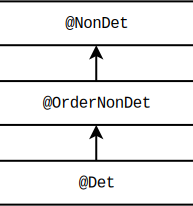
\includegraphics[scale=0.5]{determinism}
	\end{center}
	\caption{Determinism type hierarchy}
	\label{fig-determinism-hierarchy}
\end{figure}

\subsection{Additional typing rules for collection elements}
Lists, set and maps - element types have to be subtypes of collection type 
Explain iterator and extracting elements of an ordernondet collection here
Examples of valid and invalid types

\subsection{Avoid aliasing unsoundness}
Give an example of unsoundness 
Recall CLIMB-to-top rule and defaulting choice for local collections (to avoid too many warnings)
Required user annotations for collections and arrays

\subsection{Special cases of polymorphism}
Explain polymorphism first
Explain modifiers to Polymorphic annotations
Poly up and down for ordernondetermistic types
Poly use for avoiding polluting det/ordernondet collections
Subtype hierarchy among all variants of Poly
Possibility of type refinement?	

\subsection{Discussion on defaulting rules}
Choice of defaults on class type, constructors and method params and return types

\subsection{Additional hardcoded rules for precision}
Example: equals on HashSet
Discussion on System properties - env, line, file and path separator.

\subsection{Annotating more classes/providing more specifications}
Ease of annotating more JDk classes
User provided stub files to override existing behavior
